% Szglab4
% ===========================================================================
%
\chapter{Grafikus felület specifikációja}

\thispagestyle{fancy}

\section{A grafikus interfész}
\comment{A menürendszer, a kezelői felület grafikus képe. A grafikus felület megjelenését, a használt ikonokat, stb screenshot-szerű képekkel kell bemutatni. Az építészetben ez a homlokzati terv.}

\begin{figure}[h]
\begin{center}
%\includegraphics[width=17cm]{chapters/chapter11/example.pdf}
\caption{x}
\label{fig:Grafikus}
\end{center}
\end{figure}

\section{A grafikus rendszer architektúrája}
\comment{A felület működésének elve, a grafikus rendszer architektúrája (struktúra diagramok). A struktúra diagramokon a prototípus azon és csak azon osztályainak is szerepelnie kell, amelyekhez a grafikus felületet létrehozó osztályok kapcsolódnak.}

\subsection{A felület működési elve}
\noindent A grafikus felület \textbf{pull} alapú működést valósít meg, tehát mindig a felület megjelenítéséért felelős objektumok fogják lekérdezni a modell aktuális állapotát. 

\noindent Ezen új, a megjelenítést szolgáló objektumok adapterként szolgálnak a modell megfelelő elemeihez: minden megjeleníteni kívánt típushoz definiálni kell egy megjelenítőt (ezután: \textbf{Sprite}), ami képes visszaadni egy adott modellobjektum vizuális reprezentációját. 

\noindent A \textbf{Spriteokat} gyűjtőosztályok
foglalják magukba, amelyek létre tudják hozni a megfelelő \textbf{Spriteokat}, valamint képesek egy modellbeli absztrakt osztály vagy interfész (\textbf{Agent}, \textbf{Field} vagy \textbf{Buff}) grafikus reprezentációjának előállítására. 

\noindent A tényleges rajzolást egy osztály végzi, amely a képrenyőre rajzolja az összes, a gyűjtőosztályok által előállított képet.

\subsection{A felület osztály-struktúrája}
\comment{Osztálydiagram. Minden új osztály, és azon régiek, akik az újakhoz közvetlenül kapcsolódnak.}

\section{A grafikus objektumok felsorolása}

\subsection{AgentElementSprite}
\begin{itemize}
\item Felelősség \newline
    Az \textbf{Agent} absztrakt osztály leszármazott osztályainak grafikus reprezentációját állítja elő.
\item Ősosztályok
\item Interfészek
    \begin{itemize}
        \item AgentVisitor
        \item SpriteHandle
    \end{itemize}
\item Attribútumok
    \begin{itemize}
        \item -agent: Agent: az \textbf{Agent}, amelyikre az osztály vonatkozik
        \item -agentSprite: SpriteHandle: az \textbf{Agentnek} megfelelő \textbf{Sprite}
    \end{itemize}
\item Metódusok
	\begin{itemize}
        \item Agent getAgent(): visszaadja az osztály által kezelt \textbf{Agent} példányt
	\end{itemize}
\end{itemize}

\subsection{BuffElement}
\begin{itemize}
\item Felelősség \newline
    Ez az interfész előírja, hogy az őt implementáló osztályoknak képesnek kell lenniük \textbf{BuffVisitorok} fogadására. 
\item Ősosztályok
\item Interfészek
\item Attribútumok
\item Metódusok
	\begin{itemize}
        \item void accept(visitor: BuffVisitor): ez a metódus képes a \textbf{BuffVisitorok} fogadására
	\end{itemize}
\end{itemize}

\subsection{BuffElementSprite}
\begin{itemize}
\item Felelősség \newline
    A \textbf{Buff} absztrakt osztály leszármazott osztályainak grafikus reprezentációját állítja elő.
\item Ősosztályok
\item Interfészek
    \begin{itemize}
        \item BuffVisitor
        \item SpriteHandle
    \end{itemize}
\item Attribútumok
    \begin{itemize}
        \item -buff: Buff: a \textbf{Buff}, amelyikre az osztály vonatkozik
        \item -buffSprite: SpriteHandle: az \textbf{Buffnak} megfelelő \textbf{Sprite}
    \end{itemize}
\item Metódusok
	\begin{itemize}
        \item Buff getBuff(): visszaadja az osztály által kezelt \textbf{Buff} példányt
	\end{itemize}
\end{itemize}

\subsection{BuffVisitor}
\begin{itemize}
\item Felelősség \newline
    Ezen interfészt implementáló osztályok képessé válnak a \textbf{BuffElement} absztrakt osztály leszármazott osztályainak elérésére azoknak publikus interfészén keresztül.
\item Ősosztályok
\item Interfészek
\item Attribútumok
\item Metódusok
	\begin{itemize}
        \item void visit(element: Oil): egy \textbf{Oil} objektum elérésére képes annak publikus interfészén keresztül
        \item void visit(element: Sticky): egy \textbf{Sticky} objektum elérésére képes annak publikus interfészén keresztül
	\end{itemize}
\end{itemize}

\subsection{EmptyFieldCellSprite}
\begin{itemize}
\item Felelősség \newline
    Egy \textbf{EmptyFieldCell} grafikus reprezentációját állítja elő
\item Ősosztályok
\item Interfészek
    \begin{itemize}
        \item SpriteHandle
    \end{itemize}
\item Attribútumok
    \begin{itemize}
        \item -model: EmptyFieldCell: az osztály által kezelt \textbf{EmptyFieldCell}
        \item -image: BufferedImage (static): az osztály grafikus reprezentációját tartalmazó kép
    \end{itemize}
\item Metódusok
\end{itemize}

\subsection{FieldCellSprite}
\begin{itemize}
\item Felelősség \newline
    Egy \textbf{FieldCell} grafikus reprezentációját állítja elő
\item Ősosztályok
\item Interfészek
    \begin{itemize}
        \item SpriteHandle
    \end{itemize}
\item Attribútumok
    \begin{itemize}
        \item -model: FieldCell: az osztály által kezelt \textbf{FieldCell}
        \item -image: BufferedImage (static): az osztály grafikus reprezentációját tartalmazó kép
    \end{itemize}
\item Metódusok
\end{itemize}

\subsection{FieldElementSprite}
\begin{itemize}
\item Felelősség \newline
    A \textbf{Field} absztrakt osztály leszármazott osztályainak grafikus reprezentációját állítja elő.
\item Ősosztályok
\item Interfészek
    \begin{itemize}
        \item FieldVisitor
        \item SpriteHandle
    \end{itemize}
\item Attribútumok
    \begin{itemize}
        \item -field: Field: a \textbf{Field}, amelyikre az osztály vonatkozik
        \item -fieldSprite: SpriteHandle: az \textbf{Fieldnek} megfelelő \textbf{Sprite}
    \end{itemize}
\item Metódusok
	\begin{itemize}
        \item Field getField(): visszaadja az osztály által kezelt \textbf{Field} példányt
	\end{itemize}
\end{itemize}

\subsection{FinishLineFieldCellSprite}
\begin{itemize}
\item Felelősség \newline
    Egy \textbf{FinishLineFieldCell} grafikus reprezentációját állítja elő
\item Ősosztályok
\item Interfészek
    \begin{itemize}
        \item SpriteHandle
    \end{itemize}
\item Attribútumok
    \begin{itemize}
        \item -model: FinishLineFieldCell: az osztály által kezelt \textbf{FinishLineFieldCell}
        \item -image: BufferedImage (static): az osztály grafikus reprezentációját tartalmazó kép
    \end{itemize}
\item Metódusok
\end{itemize}

\subsection{GameGraphics}
\begin{itemize}
\item Felelősség \newline
    A \textbf{Spriteok} által előállított képek kirajzolása a képernyőre.
\item Ősosztályok
    \begin{itemize}
        \item jawax.swing.JPanel
    \end{itemize}
\item Interfészek
    \begin{itemize}
        \item jawa.awt.image.ImageObserver
    \end{itemize}
\item Attribútumok
    \begin{itemize}
        \item -bufferedImage: BufferedImage: a teljes kirajzolandó kép
        \item -map: game.Map: a kirajzolandó pálya
        \item -drawableFields: Map<Field, FieldElementSprite>: mapping a pálya \textbf{Fieldjei} és a grafikáért felelős \textbf{FieldElementSpriteok} között
    \end{itemize}
\item Metódusok
	\begin{itemize}
        \item bool attachToMap(map: game.Map): beállítja, hogy melyik pályát akarjuk kirajzolni
        \item void centerFieldTo(center: Field, radius: int): kirajzol egy NxM-es területet a megadott \textbf{Field} körül, ahol minden \textbf{Field} radius nagyságú
	\end{itemize}
\end{itemize}

\subsection{OilSprite}
\begin{itemize}
\item Felelősség \newline
    Egy \textbf{Oil} grafikus reprezentációját állítja elő
\item Ősosztályok
\item Interfészek
    \begin{itemize}
        \item SpriteHandle
    \end{itemize}
\item Attribútumok
    \begin{itemize}
        \item -model: Oil: az osztály által kezelt \textbf{Oil}
        \item -image: BufferedImage (static): az osztály grafikus reprezentációját tartalmazó kép
    \end{itemize}
\item Metódusok
\end{itemize}

\subsection{RobotSprite}
\begin{itemize}
\item Felelősség \newline
    Egy \textbf{Robot} grafikus reprezentációját állítja elő
\item Ősosztályok
\item Interfészek
    \begin{itemize}
        \item SpriteHandle
    \end{itemize}
\item Attribútumok
    \begin{itemize}
        \item -model: Robot: az osztály által kezelt \textbf{Robot}
        \item -startColorIndex: int (static): a \textbf{Robot} példányainak megkülönböztetésére használt statikus index
        \item -colorIndex: int: az aktuális \textbf{Robot} színének meghatározására használt index
    \end{itemize}
\item Metódusok
\end{itemize}

\subsection{SpriteHandle}
\begin{itemize}
\item Felelősség \newline
    Az interfészt implementáló osztályoknak elő kell tudniuk állitani saját grafikus reprezentációjukat
\item Ősosztályok
\item Interfészek
\item Attribútumok
\item Metódusok
	\begin{itemize}
        \item BufferedImage getItemImage(): visszaadja az implementáló osztály grafikus reprezentációját
	\end{itemize}
\end{itemize}

\subsection{StickySprite}
\begin{itemize}
\item Felelősség \newline
    Egy \textbf{Sticky} grafikus reprezentációját állítja elő
\item Ősosztályok
\item Interfészek
    \begin{itemize}
        \item SpriteHandle
    \end{itemize}
\item Attribútumok
    \begin{itemize}
        \item -model: Sticky: az osztály által kezelt \textbf{Sticky}
        \item -image: BufferedImage (static): az osztály grafikus reprezentációját tartalmazó kép
    \end{itemize}
\item Metódusok
\end{itemize}

\subsection{VacuumSprite}
\begin{itemize}
\item Felelősség \newline
    Egy \textbf{Vacuum} grafikus reprezentációját állítja elő
\item Ősosztályok
\item Interfészek
    \begin{itemize}
        \item SpriteHandle
    \end{itemize}
\item Attribútumok
    \begin{itemize}
        \item -model: Vacuum: az osztály által kezelt \textbf{Vacuum}
        \item -image: BufferedImage (static): az osztály grafikus reprezentációját tartalmazó kép
    \end{itemize}
\item Metódusok
\end{itemize}

\section{Kapcsolat az alkalmazói rendszerrel}

A következő diagramon látható, hogy miképpen tudja meg a GameGraphics osztály, hogy milyen típusú Field-et kell rajzoljon egy adott helyre. Ugyanígy derül ki a program egy mélyebbik pontján, hogy milyen típusú Agent és Buff van egy adott Field-en. Mindezt Visitor pattern segítségével oldjuk meg. 
A FieldElementSprite FieldVisitorként megtudja, hogy a fieldSprite tagváltozójának milyen értéket adjon.

\begin{figure}[h]
    \begin{center}
        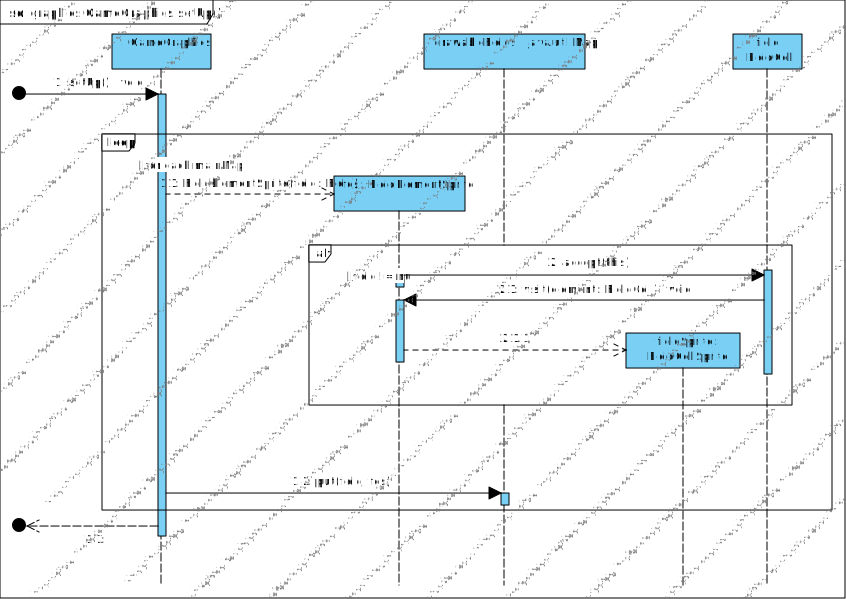
\includegraphics[width=\textwidth]{chapters/chapter11/fieldbeallitas.pdf}
        \caption{Egy Field beállítása}
        \label{fig:fieldbeallitas}
    \end{center}
\end{figure}


Ezen a diagramon egy Rajzolási szekvencia látható. Itt arra fektetünk hangsúlyt, hogy miképpen kérdezi le egy Field a rajtalévő elemeket és hogy azokat, hogyan rajzoljuk egymásra. A félkövér-dölttel jelzett metódushívások a tényleges rajzolásokat hivatottak jelölni.

\begin{figure}[h]
    \begin{center}
        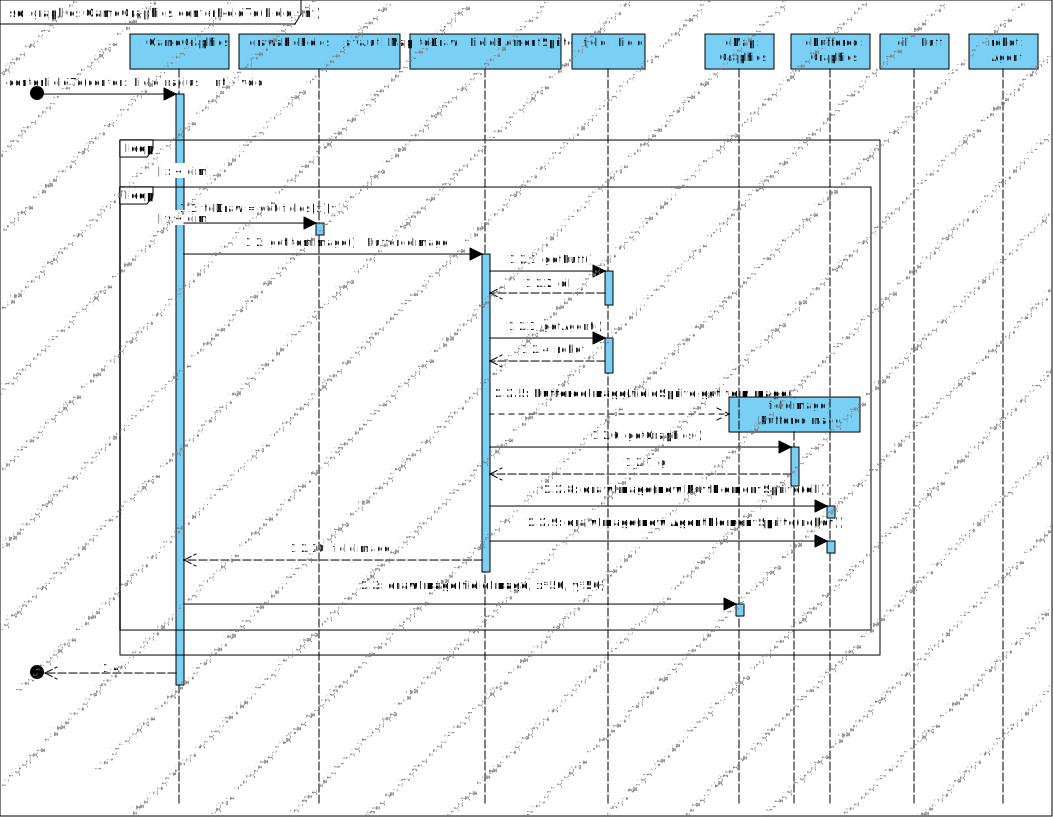
\includegraphics[width=\textwidth]{chapters/chapter11/rajzolas.pdf}
        \caption{Rajzolási szekvencia}
        \label{fig:rajzolas}
    \end{center}
\end{figure}